\chapter{Results}
\label{cha:results}


This chapter discusses the basic findings of the analysis of the proposed peer influence model.
All results were obtained from synthetic networks that were generated over \( T = 75,000 \) iterations.
The size of the networks was fixed to \(n = 5,000 \) nodes and since the model heavily depends on events that happen at random are the reported properties of the time-varying networks obtained by averaging the results of 40 independent runs.
The model parameter that are responsible for the formation of the community structures are set to \( p_{\Delta} = 0.90 \) for the triadic closure probability, \( \delta = 1 \) for the link reinforcement constant, and \( p_{d} = \num{5e-05} \) for the node deletion probability for every experiment.
Furthermore, the critical peer influence threshold was fixed to \( \theta = 0.10 \).
This reflects the idea that only a relatively small number of active neighbors is sufficient to increase the activity of a node in a significant way.

The topological properties of the integrated network, which are discussed in \cref{sec:integrated-network-properties}, are measured only for nodes that are part of the temporal network.
This means that nodes that were removed earlier due to the node deletion process do not influence the properties of the integrated network any more.
\Cref{sec:network-activity} contains an overview of the overall network activity with respect to different levels of peer influence.
The effect of the peer influence mechanism on the inter-event time distribution in the network is examined in \cref{sec:inter-event-time-dists}.
All this experiments are performed for different values for the maximum peer influence probability \( q \).
However, the last section (\cref{sec:softmax-rescaling}) keeps the peer influence level constant and discusses how different values for \( \beta \), the inverse temperature for the softmax weight re-scaling, change the peer influence effects in the network.
The synthetic networks that are used in the first three sections use the average tie strength as temperature for the softmax weight re-scaling.
Therefore, \( \beta \) is set to the to the inverse of the average of the weights in the integrated network in each iteration after the first one.
The value is set to \( \beta = 1 \) in the initial round to avoid division by zero, due to the fact that the network is completely disconnected in the beginning.


%% ========================================================================
%% ========================================================================


\section{Integrated Network Properties}
\label{sec:integrated-network-properties}

Not only the integrated network of all 75,000 previous instantaneous networks and its properties are of great interest, but also how they evolve during the simulation.
This allows to get a deeper understanding on how the model shapes the community structures in the network.
To make this possible is the integrated network build in an iterative fashion.
A snapshot of it is taken after the newly formed ties are added and the weights of already established links are updated in every time step.
Features like the average local clustering coefficient or the average weight of the ties are then calculated for all of the 75,000 integrated network snapshots.
This allows to examine on how the topology and other measures change over time.

The first, and most interesting, measure that can be investigated in this way is the average local clustering coefficient \( C(t) \).
\Cref{fig:avg-local-cc-full} depicts the development of it over the course of the simulation for different levels of peer influence.
The graph of this function has a very distinctive pattern, which was already explained in the original work by \citet{Laurent2015}.
The average clustering coefficient is very small in the first few hundred iterations, due to the sparsity of the integrated network.
Almost all nodes are disconnected and the number of triangles that have formed is relatively small compared to the size of the network.
However, \cref{fig:avg-local-cc-full} also shows that the clustering coefficient grows very fast until it reaches its maximum value, depending on the level of peer influence, between 3,000 and 5,000 iterations.
This rapid increase is caused by the cyclic closure mechanism of the model.
Nodes that become active in this early state first have to introduce some ties with nodes that were selected using the focal closure mechanism.
This does not increase the average local clustering coefficient in a significant way, however, it establishes the egocentric networks.
After the first triangles are closed, the first strong ties start to develop.
These emerging strong ties amplify the biased local search of the triadic closure mechanism and result, on one hand, in in more triangles, and on the other hand, in the reinforcement of already established triangles and the associated strong ties.
This leads to a high local clustering in the established communities.
However, weak ties are also introduced by the focal closure mechanism during the simulation.
They are rarely involved in the formation of new triangles, due to the bias towards strong ties, which contributes to the decrease of the average local clustering coefficient until the network reaches its stationary state.
The percentage of network activity that is responsible for the reinforcement of ties in each iteration \( r(t) \) supports this behavior as well.
In the beginning most activity is spend on forming new ties and therefore building the topological structures of the network, but after a while \( r(t) \) increases drastically and converges to a value of over 90\%, which indicates the domination of the reinforcement process (c.f. \cref{fig:percentage-reinforced-ties}).


\myfig{avg-local-cc-full}
      {width=0.75\textwidth}
      {The average local clustering coefficient \( C \) as a function of time for different maximum peer influence probabilities \( q = 0, \, 0.01, \, 0.05, \, 0.1, \, 0.15\). }
      {Average local clustering coefficient as function of time}
      {fig:avg-local-cc-full}


\begin{figure}[htbp]
\centering
\begin{subfigure}[b]{0.485\textwidth}
  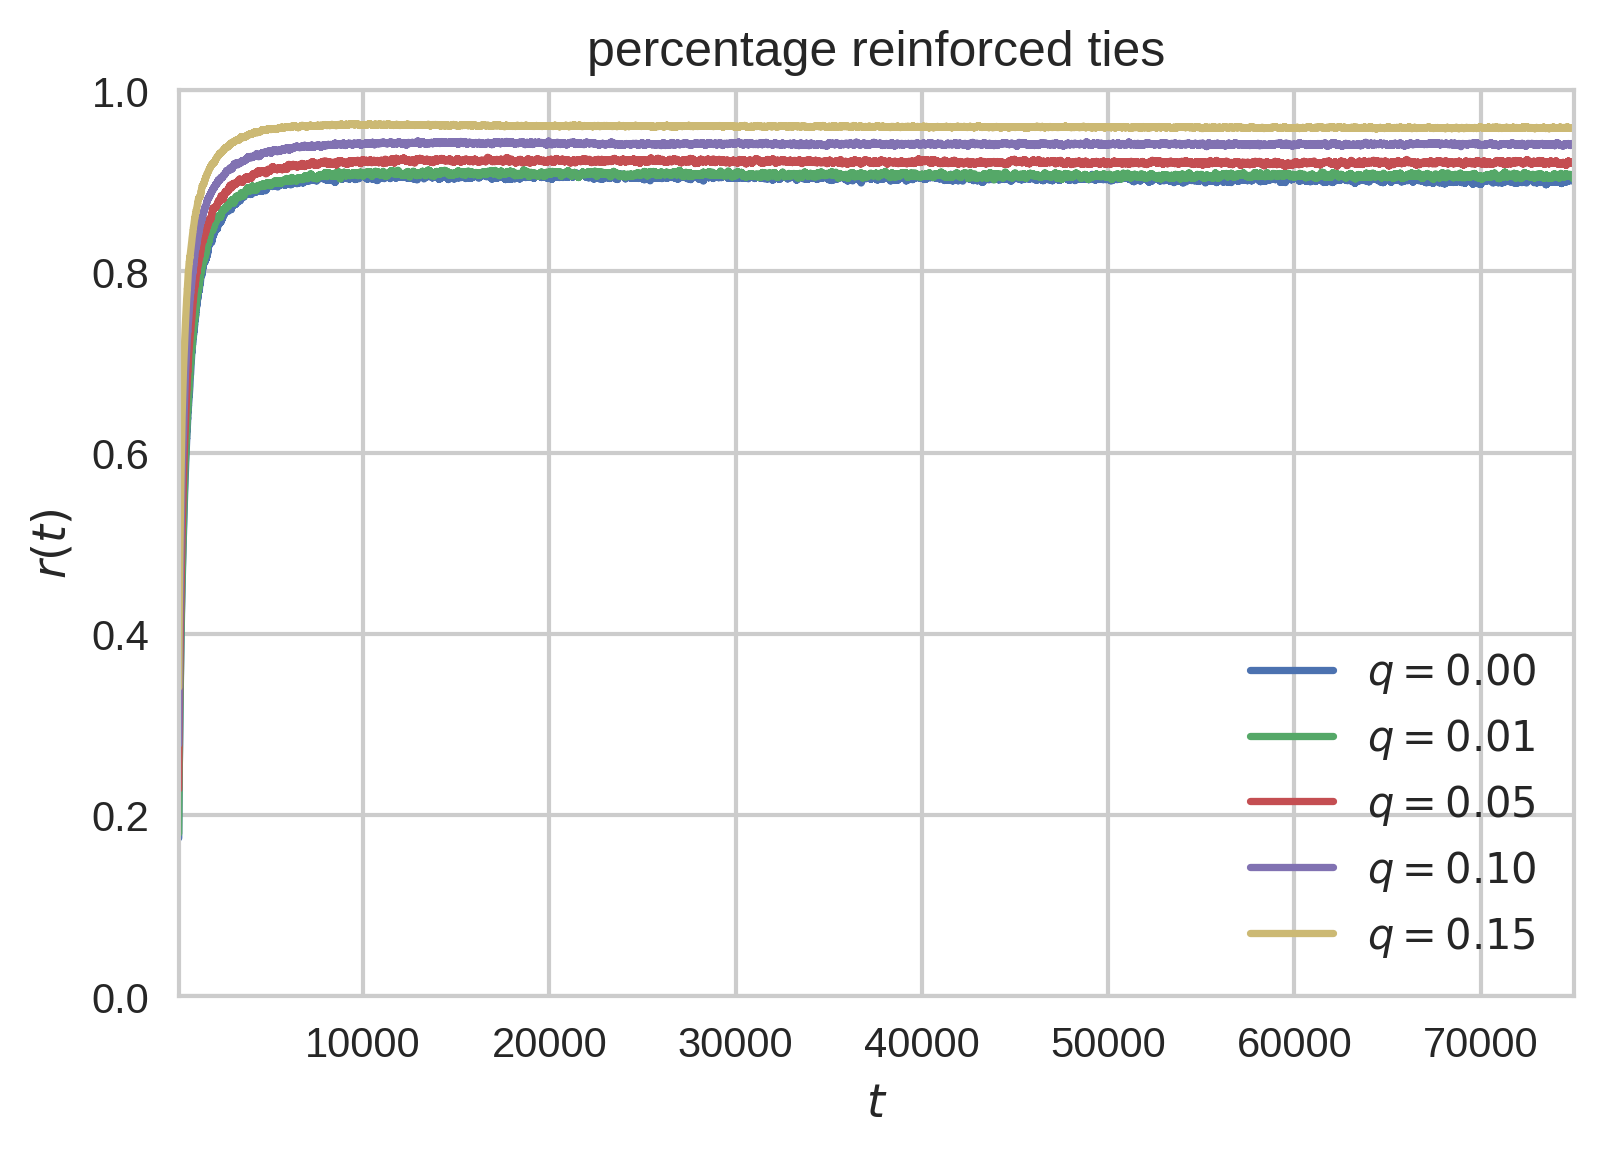
\includegraphics[width=\textwidth]{figures/percentage-reinforced-ties-full}
  \caption{}
  \label{fig:percentage-reinforced-ties-full}
\end{subfigure}
~
\begin{subfigure}[b]{0.485\textwidth}
  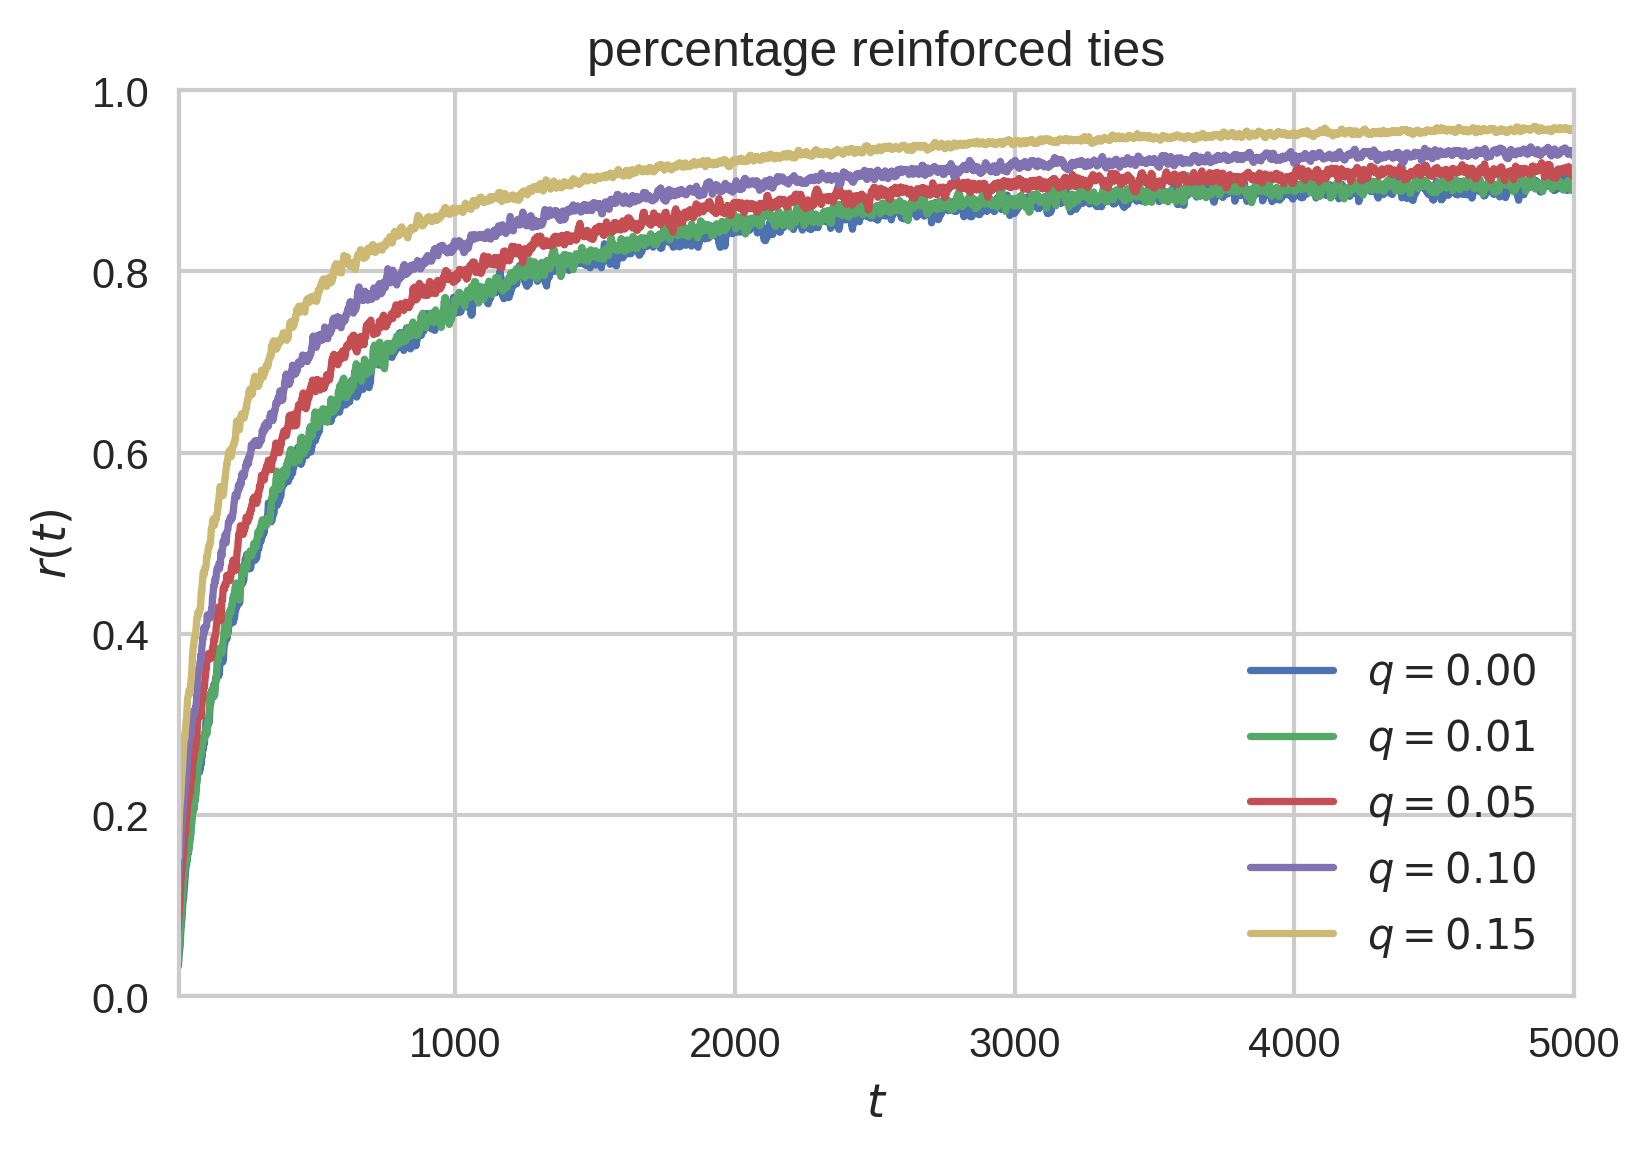
\includegraphics[width=\textwidth]{figures/percentage-reinforced-ties-beginning}
  \caption{}
  \label{fig:percentage-reinforced-ties-beginning}
\end{subfigure}

\caption[Percentage of reinforced ties as function of time]{The percentage of reinforced ties \( r(t) = \frac{\#e_{r}(t)}{\#e_{r}(t) + \#e_{c}(t)} \) for different levels of peer influence as a function of time, where \( \#e_{c}(t) \) and \( \#e_{r}(t) \) are the number of created ties and  the number of reinforced ties in iteration \( t \), respectively. (\subref{fig:percentage-reinforced-ties-full}) shows the ratio over all 75,000 iterations and (\subref{fig:percentage-reinforced-ties-beginning}) highlights the behavior in the beginning. Both functions were smoothed using the rolling mean method to improve the quality of the plot.}
\label{fig:percentage-reinforced-ties}
\end{figure}


The evolution of the average local clustering coefficient does dependent on the used node deletion probability \( p_{d} \), due to low active nodes that are not removed fast enough and are introducing weak ties.
However, as clearly evident in \cref{fig:avg-local-cc-full}, the possible level of peer influence does influence the clustering, and therefore the community structures of the network, as well.
For example, the more likely an activation due to peer influence gets, the smaller the stationary value for \( C \) becomes.
\Cref{fig:avg-local-cc-end} highlights this effect well.
This behavior can possibly be explained in a similar way as the effect caused by the deletion probability.
However, in this case is not the slow removal of nodes responsible, but the overall increased activity.
The peer influence mechanism increases the activity in the network, especially in already formed communities, since active nodes motivate their neighbors to become active as well.
The probability for the formation of a new tie is inverse proportional to the size a nodes egocentric network.
Therefore, a active node that is already fully integrated in its community will reinforce one of its existing ties, or at least close a triangle, with high probability.
However, given enough tries such a node will eventually introduce new weak ties using the focal closure mechanism as well.
Therefore, the opportunities for the introduction of random links by active nodes increases, which leads to a smaller average local clustering in general.

\begin{figure}[htbp]
\centering
\begin{subfigure}[b]{0.485\textwidth}
  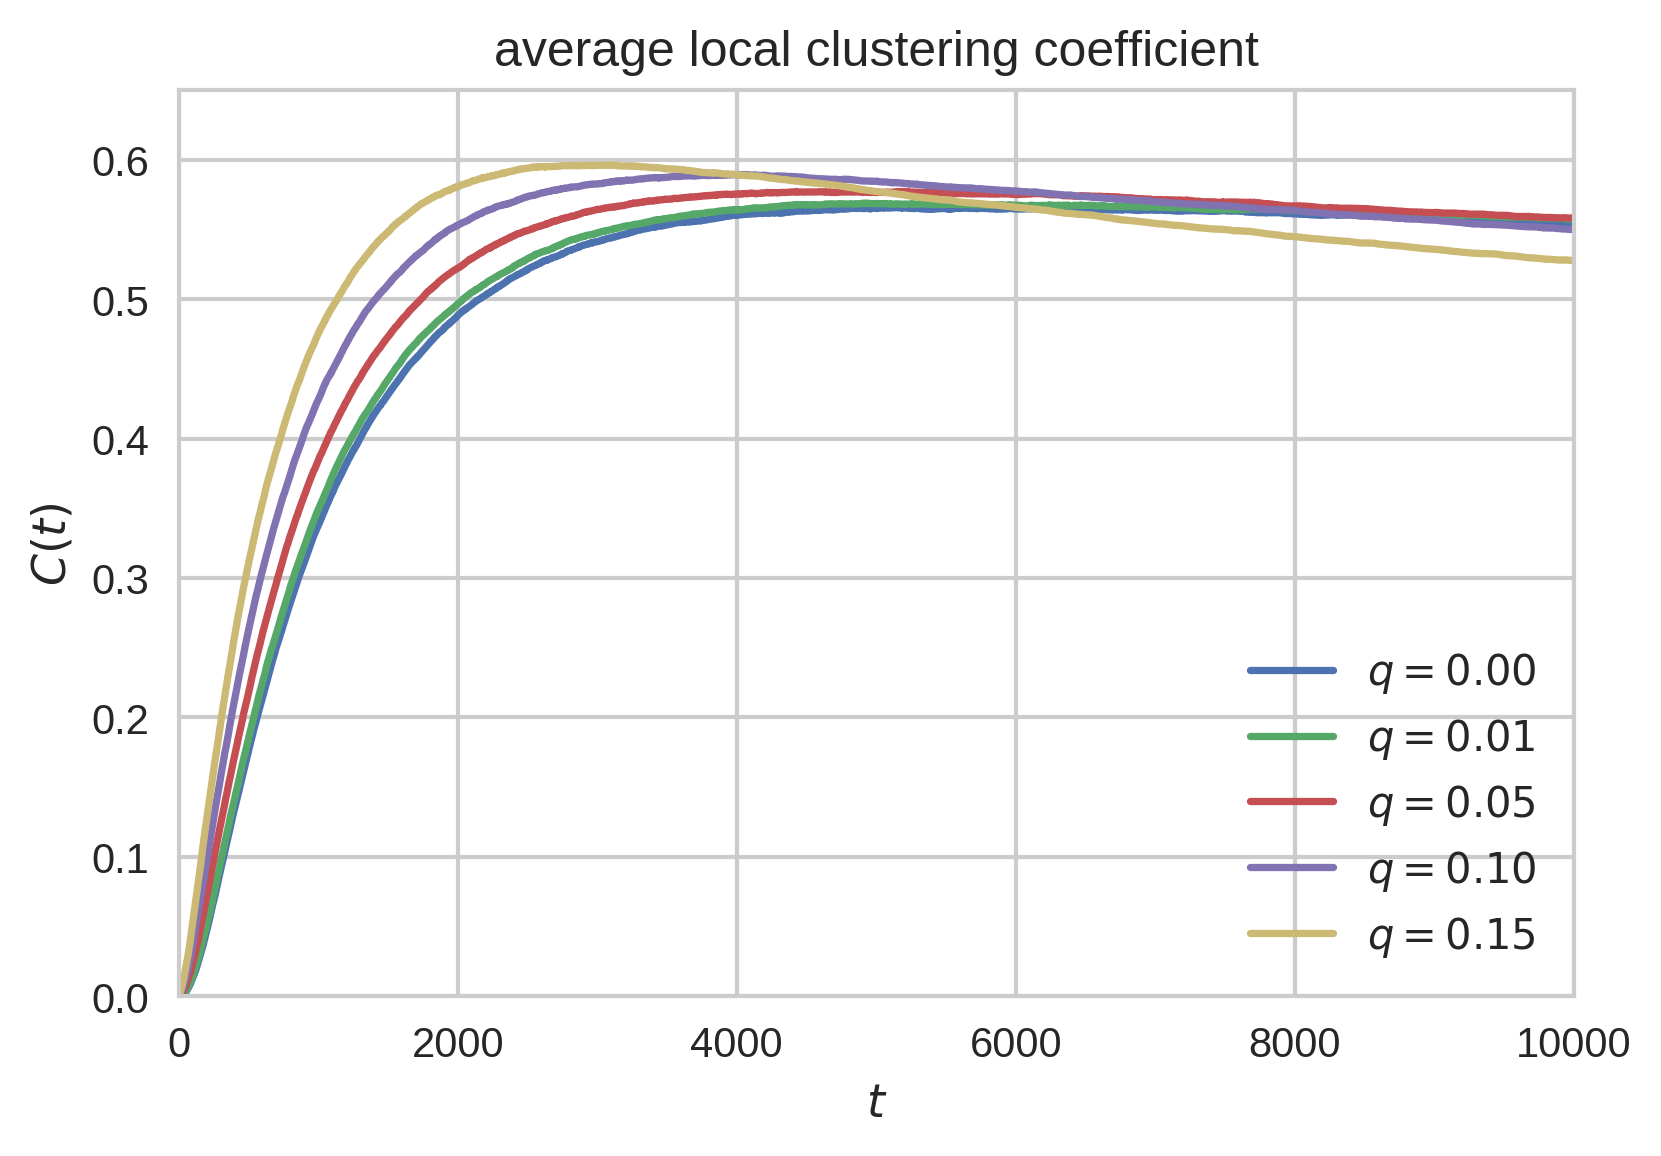
\includegraphics[width=\textwidth]{figures/avg-local-cc-start}
  \caption{}
  \label{fig:avg-local-cc-start}
\end{subfigure}
~
\begin{subfigure}[b]{0.485\textwidth}
  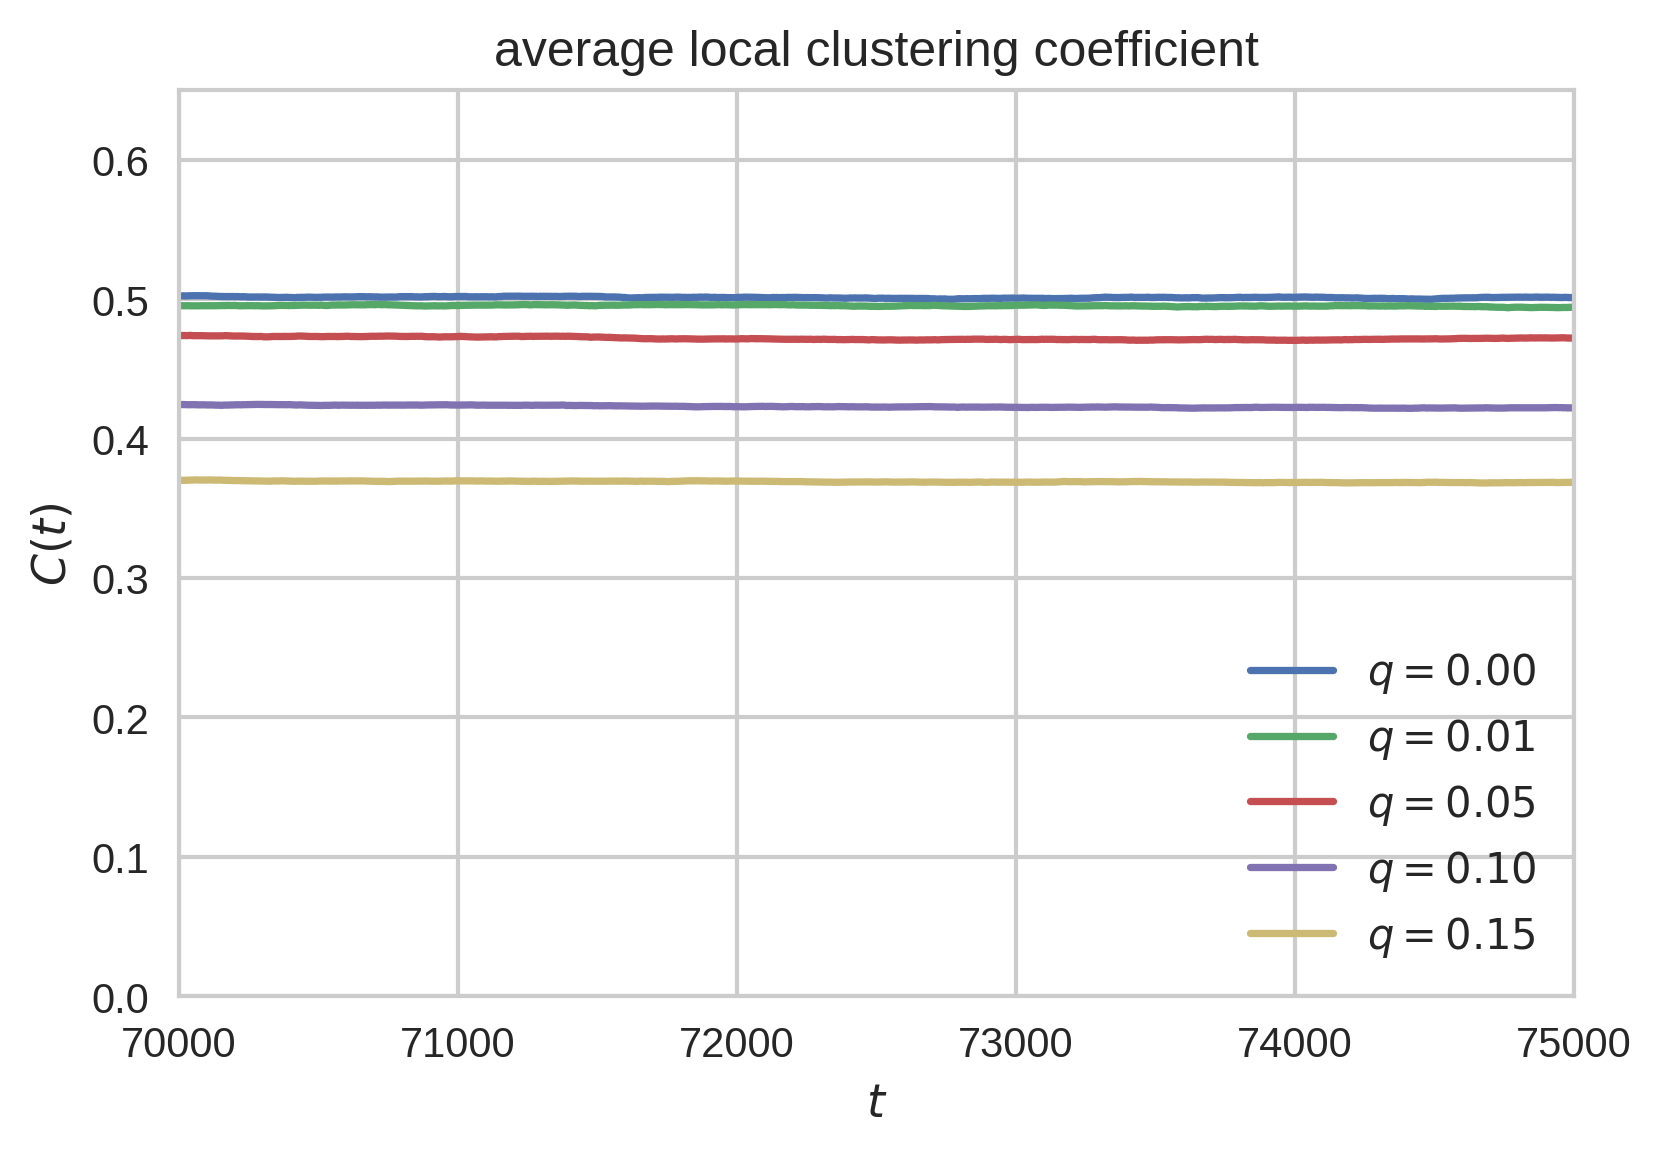
\includegraphics[width=\textwidth]{figures/avg-local-cc-end}
  \caption{}
\label{fig:avg-local-cc-end}
\end{subfigure}

\caption[Segments of the average local clustering coefficient evolution]{Segments of the evolution of the local clustering coefficient for different levels of peer influence. (\subref{fig:avg-local-cc-start}) shows the clustering coefficient for the first 10,000 iterations, in which it reaches it maximum value and slowly starts to decrease. (\subref{fig:avg-local-cc-end}) depicts the stationary values for \( C \), which can be observed in the last 5,000 iterations.}
\label{fig:avg-local-cc-details}
\end{figure}


The second effect that can be attributed to the peer influence mechanism with respect to the clustering can be observed in the initial phase of the simulation (c.f. \cref{fig:avg-local-cc-start}).
The peer influence seems to have an positive effect on the development of the topological structures in the network.
A higher level of peer influence accelerates the formation of the communities and increases the maximum value of \( C \) that is reached.


%% ========================================================================
%% ========================================================================


\section{Network Activity}
\label{sec:network-activity}


%% ========================================================================
%% ========================================================================


\section{Inter-event Time Distributions}
\label{sec:inter-event-time-dists}
% definition burstiness and parameter B is invariant wrt to activity homogeneity in \cite{Goh2008}
% nice explanation for B in \cite{Masuda2016}


%% ========================================================================
%% ========================================================================


\section{Softmax Weight Re-scaling}
\label{sec:softmax-rescaling}
